\chapter{Attacks}

In the previous chapter, we saw two basic attacks: the Fan-Out and the Nakamoto Race.
The Fan-Out is more of a misconfigured network situation, because no mining adversary
is required to mount it. The Nakamoto Race is a foundational attack.
It will function as a prototype for other attacks which we will explore in this chapter.

In this chapter, we will talk about how the various ledger virtues we defined in the
last chapter can be broken by adversaries of varying mining power. Because ledger virtues
follow from chain virtues, the adversary will have to break the chain virtues first.
So we will look at \emph{examples} of attacks that break the chain virtues. Remember,
if we describe an attack that works, this is sufficient to illustrate that the system
is broken. However, if an attack we think about happens \emph{not} to work, this is not
sufficient to argue that the system is secure. We may have just happened to think of
the wrong attack.

\section{Attacks of a Minor Adversary}\index{Minor Adversary}

A minor adversary is an adversary for which $t < n - t$. This is also known as
a $< 50\%$ attack. What virtues can such an adversary break? Let us go over all the
virtues in question and explore how much an adversary can break them.

\subsection*{Common Prefix}
As we saw in the last chapter, it is possible to have \emph{good} or
\emph{bad} configurations of the system if the parameters $T$ and $k$ are set incorrectly
when the $\Delta$, $t$, $n$, $q$ that exist on the network are taken into account.
For example, consider the extreme value
$T = 2^\kappa$. Then every query is a successful query, and every successful query
failed to be a convergence opportunity. Then, if there are multiple honest parties
$n - t > 1$, it doesn't make a difference how much we wait for $k$; we will never
have convergence. As such, Common Prefix is not achieved, and therefore safety is
violated. In these very misconfigured networks, the adversary can cause a Common
Prefix violation even with no mining power, just by allowing the honest parties
to diverge on their own.

However, in proper blockchain protocol configurations, the density of convergence
opportunities will be more than the density of adversarially successful queries.
In these cases, \emph{the best attack that a minor adversary can do is to perform the
Nakamoto Attack}~\cite{nakamoto-wins}. As we've seen, using this attack she cannot break Common Prefix,
except with negligible probability in $k$. The more we allow $k$ to grow, the more the actual successful
queries of the adversary and the actual convergence opportunities will tend to
approximate their expectations. We will make this argument precise when we
prove the Common Prefix against \emph{all} adversaries in Chapter~\ref{chapter:earnest3}.

\subsection*{Chain Growth}
Even though a minor adversary can affect the chain velocity $\tau$ of honest
parties by stopping her mining, she cannot prevent the rest of the honest network
from mining. If she is a minority adversary, this can mean she can drop the expected
chain growth rate to at worse $\frac{1}{2}$ of what it would be were she to mine honestly.
\emph{The best strategy for harming chain growth is simply not to mine}.
Even if the adversary mines withheld chains in the fashion that the Nakamoto Race
attack does, these chains will not be adopted, unless they are longer than what
the honest parties have adopted. In these cases, even though the honest parties are
switching from one chain to another, the chain they are switching to is still longer
than what they have, and so Chain Growth is happening.

\subsection*{Chain Quality}
For a minor adversary to harm Chain Quality, she would have to try and supress as many
honestly generated blocks as possible from becoming adopted by honest parties. Ideally,
she wants honest parties to adopt chains that only consist of adversarially generated blocks.

In case the adversary plays honestly, and no forks occur on the chain, then the number of
blocks she gets is proportional to her mining power. The honest adversary\footnote{The
\emph{honest adversary} is not a misnomer. Remember that the adversary controls any party which
we did not designate as honest. She can do whatever she wishes with that party -- including
playing honestly.}
therefore achieves quality $\mu = \frac{n - t}{n}$. This matches our expectation that
the proportion of blocks on a chain generated by a particular party match his mining power.

\section{Selfish Mining}
We might try to think about different strategies in which the adversary may
try to harm quality. There is an adversarial strategy known as \emph{Selfish Mining}\index{Selfish Mining}
which is a modified version of the Nakamoto Race, and specifically targets the minimization
of the quality of the honestly adopted chain.

The adversary works as follows. Initially, all honest parties start at some block $B$.
Similar to the Nakamoto Race, the honest parties and the adversary mine on separate forks,
both extending $B$. If at any point of time the adversary finds a block on her fork, she keeps
it secret, similarly to the Nakamoto Race. She can keep growing her secret fork more and more.
If at any point in time the honest parties find a block, then the adversary wishes to suppress
it from the honestly adopted chain. There are two cases: Either she has at least one withheld
block up her sleeve on her secret fork, or she does not. If, when the honest parties mine a block,
the adversary does not have a withheld block up her sleeve, then there isn't much she can do.
Since she doesn't have any secret blocks, she accepts that the honestly mined block that was
just broadcast will be accepted as part of the honestly adopted chain, and restarts mining
her secret fork on top of the honestly generated block.

On the contrary, if
she has one or more withheld blocks up her sleeve, she releases exactly \emph{one} of her
withheld blocks in an attempt
to kick out the block produced by the honest party from the honestly adopted chain. If
the adversary's block makes it to the doorstep of other honest parties before the honestly
mined block arrives, the adversarially generated block will be adopted, and the
honestly generated block will be rejected.
The adversary keeps the rest of her withheld blocks secret so that they can be used in the
future.

Whether the adversarial block can make it to the doorstep of an honest party before the
honest block makes it there is an issue of how well positioned the adversary is on the
network. Remembering our threat model, we want to make the adversary as powerful as possible,
so that, when the time comes to prove the security of our protocol, the proof of security
will be the strongest. As such, we will assume that the adversary has significantly better
network presence than the honest parties. We model this as follows. Whenever any honest party
broadcasts a message to the network, the adversary gets a chance to see it \emph{first},
prior to any other honest party seeing it. The adversary then has the choice to broadcast
her own message \emph{prior} to the honest message making its way. In this way, the adversary
can \emph{rush ahead} in her message delivery as compared to the honest message delivery.
She can \emph{frontrun} honest messages after seeing them so that adversarial messages
get delivered prior to the honest message. We call such an adversary a
\emph{Rushing Adversary}\index{Rushing Adversary}. This may seem like giving too much power
to the adversary, but is not an unreasonable assumption in practice. When we deploy our real
systems, we want to give assurances to honest parties even if they have very basic network
connectivity, for example through a slow Internet connection in a remote area. On the contrary,
it is rather inexpensive for the adversary to buy good network presence by deploying some
servers on central Internet backbone locations. This would allow the adversary to actually
mount rushing attacks against parties located on the Internet's last mile quite successfully.

% TODO: algorithm for the selfish miner

The basic idea of the selfish ming attack is that, whenever the adversary has a headstart of secretly
kept blocks, any honest mining power goes to waste, because any blocks produced by the honest
parties during those moments will be kicked out by the competing blocks broadcast by the rushing
adversary.

This is a more complicated attack than what we've seen before, so let's look at an example
execution of the attack. The example is illustrated in Figure~\ref{fig.selfish-mining}. The
honestly generated blocks are colored blue, while the adversarially generated blocks are
colored red. The final honestly adopted chain is displayed at the bottom and consists of a
mixture of honestly generated and adversarially generated blocks, whereas abandoned honest
blocks are seen at the top as temporary forks. The blocks are numbered in the order they were
mined. As you can see, adversarially mined blocks are never abandoned. The only blocks ever
abandoned are honestly mined. Additionally, all temporary forks have a length of exactly $1$.
The example begins with everyone having genesis. Initially, both the adversary and the honest
parties attempt to mine a block on top of genesis. An honest party manages to get a block first,
and this is block $1$. As the adversary does not hold any withheld blocks, she adopts block
$1$, and so does every other honest party. Now the honest parties and the adversary all mine
on top of block $1$. At this point, the adversary manages to get block $2$, but keeps it secret.
Now the adversary is mining on top of block $2$, but the honest parties are mining on top of
block $1$. At this point, the adversary gets lucky and manages to mine another block $3$
on top of block $2$. She keeps both block $2$ and block $3$ secret. Now the adversary is mining
on top of block $3$, but the honest parties are still mining on top of block $1$. An honest
party manages to get block $4$ and broadcasts it to the network. The adversary
sees this block being broadcast on the network and rushes to send her own block $2$ in order to
suppress honest block $4$. Since the adversary is rushing, she manages to get block $2$ on
the doorstep of every honest party prior to them seeng block $4$. Therefore every honest
party (beyond the one who mined block $4$) now adopts block $2$ and keeps mining on top of it.
Note how the honest mining power that went into mining block $4$ went completely to waste
here, because the adversary knew ahead of time that she would be able to replace this block.
Now every honest party is mining on top of block $2$, but the adversary is still ahead and
mining on top of block $3$. The honest parties generate block $5$, but the adversary counters
by releasing block $3$. At this point, both the honest parties and the adversary have adopted
and are mining on top of block $6$, and the adversary has no headstart any more.

The honest parties manage to get block $8$, which the adversary is forced to accept, since she
has no withheld blocks at this time. Next, she gets $9$ and keeps it secret. The honest parties
get $10$, but the adversary uses $9$ to suppress it. At this point, both the honest parties
and the adversary are mining on $9$. The adversary gets $11$. The honest parties get $12$ and
the adversary suppresses it with $11$. The honest parties get $13$, which the adversary accepts.
Next, the adversary gets $14$. The honest parties get $15$, and the adversary suppresses it with
$14$. Lastly, the honest parties get $16$ and everybody adopts it.

\begin{figure}[h]
    \centering
    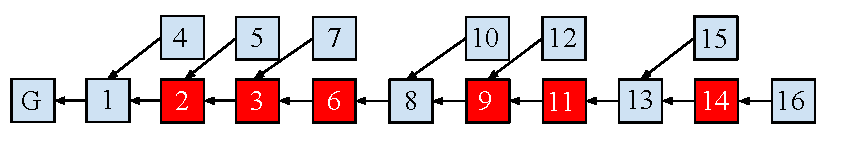
\includegraphics[width=\columnwidth,keepaspectratio]{figures/selfish-mining.pdf}
    \caption{The selfish mining attack in action. Red blocks (2, 3, 6, 9, 12, 14) are adversarially
             generated, whereas blue blocks are honestly generated.}
    \label{fig.selfish-mining}
\end{figure}

We wish to discover how low the chain quality $\mu$ gets for various values of
$\frac{t}{n}$. This attack seems harder to analyze analytically, so we will use a simulation
method to analyze its efficiency. In the simulation, we will code a simplified model of the attack
in which the honest parties only get convergence opportunities, and there are no successful queries
that are not convergence opportunities. This gives an advantage
to the honest parties, so, if our adversary is successful against these honest
parties, she is definitely going to also be successful against more modest honest parties
who also have to deal with the lack of convergence opportunities. We use this simplification
because we consider temporary forks due to network desynchronization immaterial to the attack in
question, and we want to get an approximate feeling for how the chain quality behaves.

The pseudocode for the simulation is illustrated in Algorithm~\ref{alg.selfish-simulation}.

\import{./}{algorithms/alg.selfish-simulation}

% TODO...

\section{Attacks of a Majority Adversary}\index{Major Adversary}
\section{Healing}

\chapter{The Selfish Miner \small{\textsf{DRAFT}}}

\section{Attacks of a Minority Adversary}
A common conjecture is that Chain Quality can be approximated by the fraction of mining power that honest parties (however, future lectures will reveal that this is not the case).

% Common prefix is broken if the adversary releases its chain to only a subset of nodes, thus making prefixes inconsistent until honest parties gossip amongst themselves. Chain quality is broken since a significant portion of the released chain is mined by the adversary.  Virtue \#2 (chain growth) is upheld as long as there are any honest participants mining that force the adversarial chain to grow.

\subsection{Majority Adversary Attack}
Now if the adversary held the majority of mining power in a network, all she needs to do is to mine a secret chain, which can be released at any time due to having more compute power. What properties can adversary break if she holds majority of the network hash power?

Clearly, she can violate the Common Prefix property as was mentioned earlier. If honest parties agree on the longest chain containing some block $B_m$, she mines a secret chain extending from the previous block $B_{m-1}$. Once the longest chain has $k$ or more blocks after $B_m$, she releases her secret chain to some of the honest miners. Since the adversarial chain is longer than the honest chain, these honest miners adopt the adversarial chain.

Additionally, an adversary with majority hash power can break Chain Quality as follows. If a block $B_m$ is mined by an honest miner, she creates a new longest chain extending the block $B_{m-1}$. Thus, the block $B_m$ is ``replaced" by a new block mined by the adversary. We will discuss this attack in more details in the next lecture.

However, in such attacks Chain Growth is upheld as long as there are any honest participants mining that force the adversarial chain to grow.

\section{Recap of Chain Virtues}
There are 3 chain virtues that are relevant to our study:

\begin{enumerate}
    \item Common prefix with parameter $k$
    \item Chain quality with parameter $\mu$
    \item Chain growth with parameter $\tau$
\end{enumerate}


Common prefix has implications for the safety of transactions on chain. Meanwhile chain quality and chain growth affect the liveness of transactions (which refers to how much time it takes for a transaction to be confirmed after it is sent to the network).
% These are also interrelated. Chain quality implies liveness because a  transaction will be validated faster if there are more honest nodes.

\subsection{Common Prefix}

Two or more chains have a common prefix of $k$ if and only if the chains agree on all blocks except the last $k$ blocks at the end of the chains.
Chains adopted by different honest nodes satisfy the common prefix property.
The probability of violation of this property decreases exponentially as $k$ increases. The greater $k$ is, the more ``forgiving" the common prefix property is, and the longer one waits to confirm a transaction.
Common prefix property implies safety of the ledger.

\subsection{Chain Quality}
The chain adopted by any honest node contains at least $\mu$ fraction of blocks mined by honest nodes.
% (ignoring temporary forks for counting purposes). These temporary forks are not necessarily problems because they will occur even in fully honest chains.

The number of blocks mined by honest nodes in a chain is important because adoption of a chain by an honest node means it is valid (there are no double spends), but there could be a censorship attack (there are no honestly mined blocks in the chain).
This property is required for liveness as adversarially mined blocks may not contain any transactions.

\subsection{Chain Growth}
The chain adopted by an honest node grows at a rate of $\tau$ blocks per unit time. This has ramifications for how fast transactions are included in the blockchain, and hence the liveness too.
\section{Censorship Attack}
Many chain attacks fall under the umbrella of a Nakamoto race, where honest parties and the adversary race to extend the length of their respective chains. Here, we will see another kind of attack. We started with the Honest Majority Assumption (henceforth HMA) which means that honest parties have more compute power than the adversary. We will look at a censorship attack that can be carried out by the adversary when she has majority compute power.

In a censorship attack, the adversary tries to prevent a certain transaction from being confirmed. The basic idea is that when she sees a transaction $\mathsf{tx}$ in a certain block, she mines at the previous block to prevent that transaction being included in the chain.
Since the adversary has majority, she can always win the Nakamoto race and therefore replace every honest block from the longest chain.
Therefore, the transaction never enters the longest chain.
This attack breaks chain quality.
The mechanism is illustrated below.


 \begin{figure}[h!]

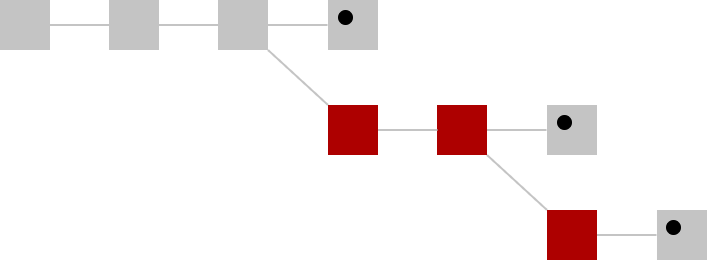
\includegraphics[scale=0.5]{figures/censorship.png}
 \caption{Depiction of a censorship attack. Grey blocks are mined by honest miners. Red blocks are valid blocks mined by the adversary. The black dot represents the transaction $\mathsf{tx}$ that the adversary is trying to censor. }
\end{figure}

\section{Attacks Under Dishonest Majority}
When honest majority holds, we have seen that the blockchain satisfies common prefix, chain quality and chain growth.
If the adversary has majority of the computing power for some time, she can break common prefix (recall the Nakamoto race attack from the previous lecture). The adversary can also break chain quality (see the censorship attack above).
However, chain growth is not broken, although it may be slowed down (i.e. the parameter $\tau$ may be reduced), because honest nodes continue to produce blocks on their longest chain.

A majority adversary can revert a transaction (by breaking common prefix). The adversary can also censor transactions (by breaking chain quality).
As a consequence, the adversary can break safety or liveness of the ledger.
However, the adversary cannot spend coins owned by an honest party because she cannot generate valid transactions for such a signature.
The adversary also cannot create more money than what is allowed by the macroeconomic policy, because such blocks would not be accepted by the honest nodes.

\section{Healing From Attacks}
Assume there is a temporary adversarial majority of compute power (TAM). Then the HMA is not respected during some time period $\delta$, and then it is respected again.
During the period of TAM, safety and liveness may not hold. The adversary can double spend and can carry out censorship attacks, violating properties like common prefix and chain quality.

After the period of TAM, when HMA is respected again, liveness heals because chain quality is recovered. Chain quality recovers because when HMA is respected, the honest parties will win the Nakamoto race and there will eventually be an honest block that includes previously censored transactions. Also, safety will heal as common prefix heals. Common Prefix recovers because of the reemergence of the HMA, and the presence of convergence opportunities means that the honest nodes will once again converge on their longest chains.

The recovery of HMA presents convergence opportunities. If convergence occurs, then any conflicting transactions which would render a block invalid (i.e. a double spend) are not included in the
honestly adopted chain
or in the mempool,
rather they are dropped.
% Chain quality heals after convergence occurrs, and honest chains are able to latch onto the same chain. Then common prefix heals when honest mining power is once more concentrated.

Since safety and liveness are not guaranteed during TAM, and it takes some time to recover safety and liveness after HMA is recovered, a user should not be using the blockchain during the TAM and a while after (if they are aware of the TAM). This is because safety and liveness cannot be recovered for coins affected during the TAM.
For example, if a car dealer delivered a car in exchange for a transaction on the blockchain during TAM, and the adversary reverted that transaction after receiving the car, that money cannot be recovered by the car dealer.


\section{Selfish Mining}
We now ask the question: Is there a lower bound on the chain quality $\mu$, and if there is, what is it? It is intuitive to guess that the lower bound is roughly the percentage of hashing power that is honest. In other words, our conjecture is that:
\begin{equation}
\label{eq:cq_conjecture}
    \mu \geq \frac{n-t}{n}
\end{equation}
We will see now that this is false. \\
Consider the selfish miner $\mathcal{A}$, who does the following:
\begin{enumerate}
    \item Adopt the longest chain
    \item Mine in secret extending the last block of the longest chain
    \item When an honest block is found:
    \begin{enumerate}
        \item If $\mathcal{A}$ has a secret block, broadcast it.
        \item Otherwise, adopt the honest tip.
    \end{enumerate}
    Then repeat from Step 2.
\end{enumerate}


Here, the adversary $\mathcal{A}$ is also a “rushing adversary”, which is one who sees honestly broadcasted messages prior to everybody else. As such, since $\mathcal{A}$ can broadcast her own block before the honest block gets to the rest of the honest miners, the honest miners will adopt $\mathcal{A}$'s block and start building the next block off of that. The honest block that $\mathcal{A}$ had originally seen is now wasted effort. If this continues, the block tree may look something like this:

\begin{figure}[h!]
\[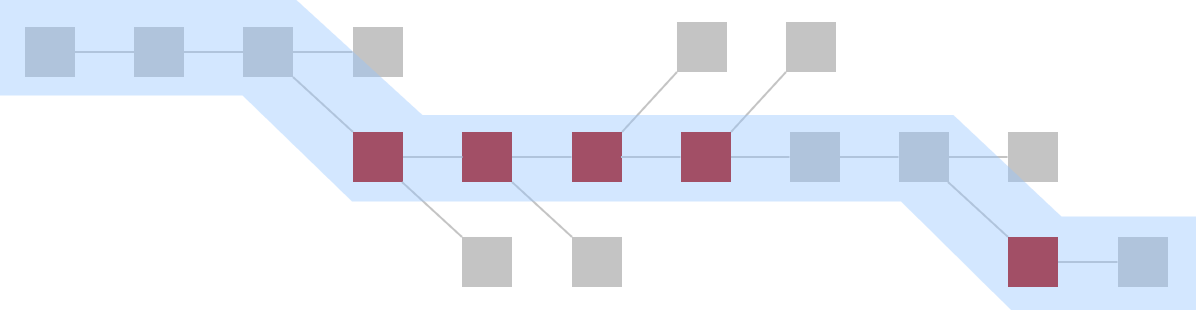
\includegraphics[scale=0.4]{figures/longestchain.png}\]
\caption{In this example, suppose that $n=17$, $t=5$ and $\frac{n-t}{n} \approx 0.71$. There are $5$ adversarial blocks and $12$ honest blocks mined which are proportional to the compute powers. In the longest chain here (highlighted in blue), there are $5$ adversarial blocks and $11$ total blocks, so we can see that $\mu \approx 0.55$. Thus, we can see that our earlier conjecture (\eqref{cq_conjecture}) is false.}
\end{figure}

Due to the wasted efforts of the honest blocks, we can start to see that $\mu$ is not necessarily equal to the fraction of honest mining power. None of the adversarial blocks are wasted in this example, but many of the honest ones are. The goal of the selfish mining attack is for every single adversarial block to be contained in the longest chain.

Below is the simulation in typescript for selfish mining. If you run it yourself, you'll see that chain quality is on average less than 0.1, even though adversarial power is 0.49.
\begin{tcolorbox}[colback=gray!30]
{\small\begin{alltt}
\begin{verbatim}
const ADVERSARIAL_POWER = 0.49
const BLOCK_LIMIT = 500
const MONTE_CARLO = 10

function simulate() {
  let honestBlocks = 1
  let adversaryHeadStart = 0
  let chainLength = 1

  while (chainLength < BLOCK_LIMIT) {
    if (Math.random() < ADVERSARIAL_POWER) {
      // adversary got a block
      ++adversaryHeadStart
    }
    else {
      // honest got a block
      if (adversaryHeadStart > 0) {
        --adversaryHeadStart
      }
      else {
        ++honestBlocks
      }
      ++chainLength
    }
  }
  return honestBlocks / BLOCK_LIMIT
}

let sumQuality = 0

for (let i = 0; i < MONTE_CARLO; ++i) {
  sumQuality += simulate()
}
console.log(sumQuality / MONTE_CARLO)
\end{verbatim}
\end{alltt}}
\end{tcolorbox}

In conclusion, an adversary does not need much mining power in order to incur heavy damage on chain quality.

\section{What Value of $T$ to Choose?}
Last class, we discussed how neither a high $T$ nor a low $T$ necessarily allows for the optimal convergence opportunity frequency. With a high $T$, blocks are produces more frequently, but they're so frequent that convergence opportunities are extremely rare. With an extremely low $T$, nearly every block is a convergence opportunity, but the blocks are so infrequent that the absolute frequency of convergence opportunities is low. So, what is the optimal $T$, you wonder? Below is the code for simulating convergence opportunity frequency with varying $T$, followed by the accompanying generated plot.
\begin{tcolorbox}[colback=gray!30]
{\small\begin{alltt}
\begin{verbatim}
import random
import matplotlib.pyplot as plt
import numpy as np

MONTE_CARLO_REPEAT = 30
TIME_INTERVAL = 100

def simulate(eta, Delta):
  convergence_opportunities = 0
  t = 0
  prev_interarrival_time = 2 * Delta
  while t < TIME_INTERVAL:
    interarrival_time = random.expovariate(1/eta)
    if interarrival_time > Delta:
      convergence_opportunities += 1
    t += interarrival_time
    prev_interarrival_time = interarrival_time
  return convergence_opportunities

def monte_carlo(eta, Delta):
  convergence_sum = 0
  for i in range(MONTE_CARLO_REPEAT):
    convergence_sum += simulate(eta, Delta)
  return convergence_sum / MONTE_CARLO_REPEAT

Delta = 1
x = []
y = []
kappa = 256
min_T_exp = 229
max_T_exp = 239
n = 10
q = 3000000
min_eta = 0.01
max_eta = 3.0
eta_step = 0.01
# eta is the expected block interarrival time
for i, eta in enumerate(np.arange(min_eta, max_eta, eta_step)):
  T = 1 / (n * q * eta)
  x.append(T)
  y.append(monte_carlo(eta, Delta))

plt.xscale('log')
plt.xlim((2**(min_T_exp - kappa), 2**(max_T_exp - kappa)))
plt.xticks(
  [2**x for x in range(min_T_exp - kappa, max_T_exp + 1 - kappa)],
  ['$2^{' + str(x) + '}$' for x in range(min_T_exp, max_T_exp + 1)]
)
plt.plot(x, y)
plt.xlabel('Mining target $T$')
plt.ylabel(f'Convergence opportunity frequency in ${TIME_INTERVAL}$ rounds')

plt.title(f'Convergence opportunities when varying the mining target $T$.
\n$\Delta = {Delta}, n = {n}, q = 3 \cdot 10^9, \kappa = {kappa}$')
plt.show()

\end{verbatim}
\end{alltt}}
\end{tcolorbox}

\begin{figure}[h!]
\[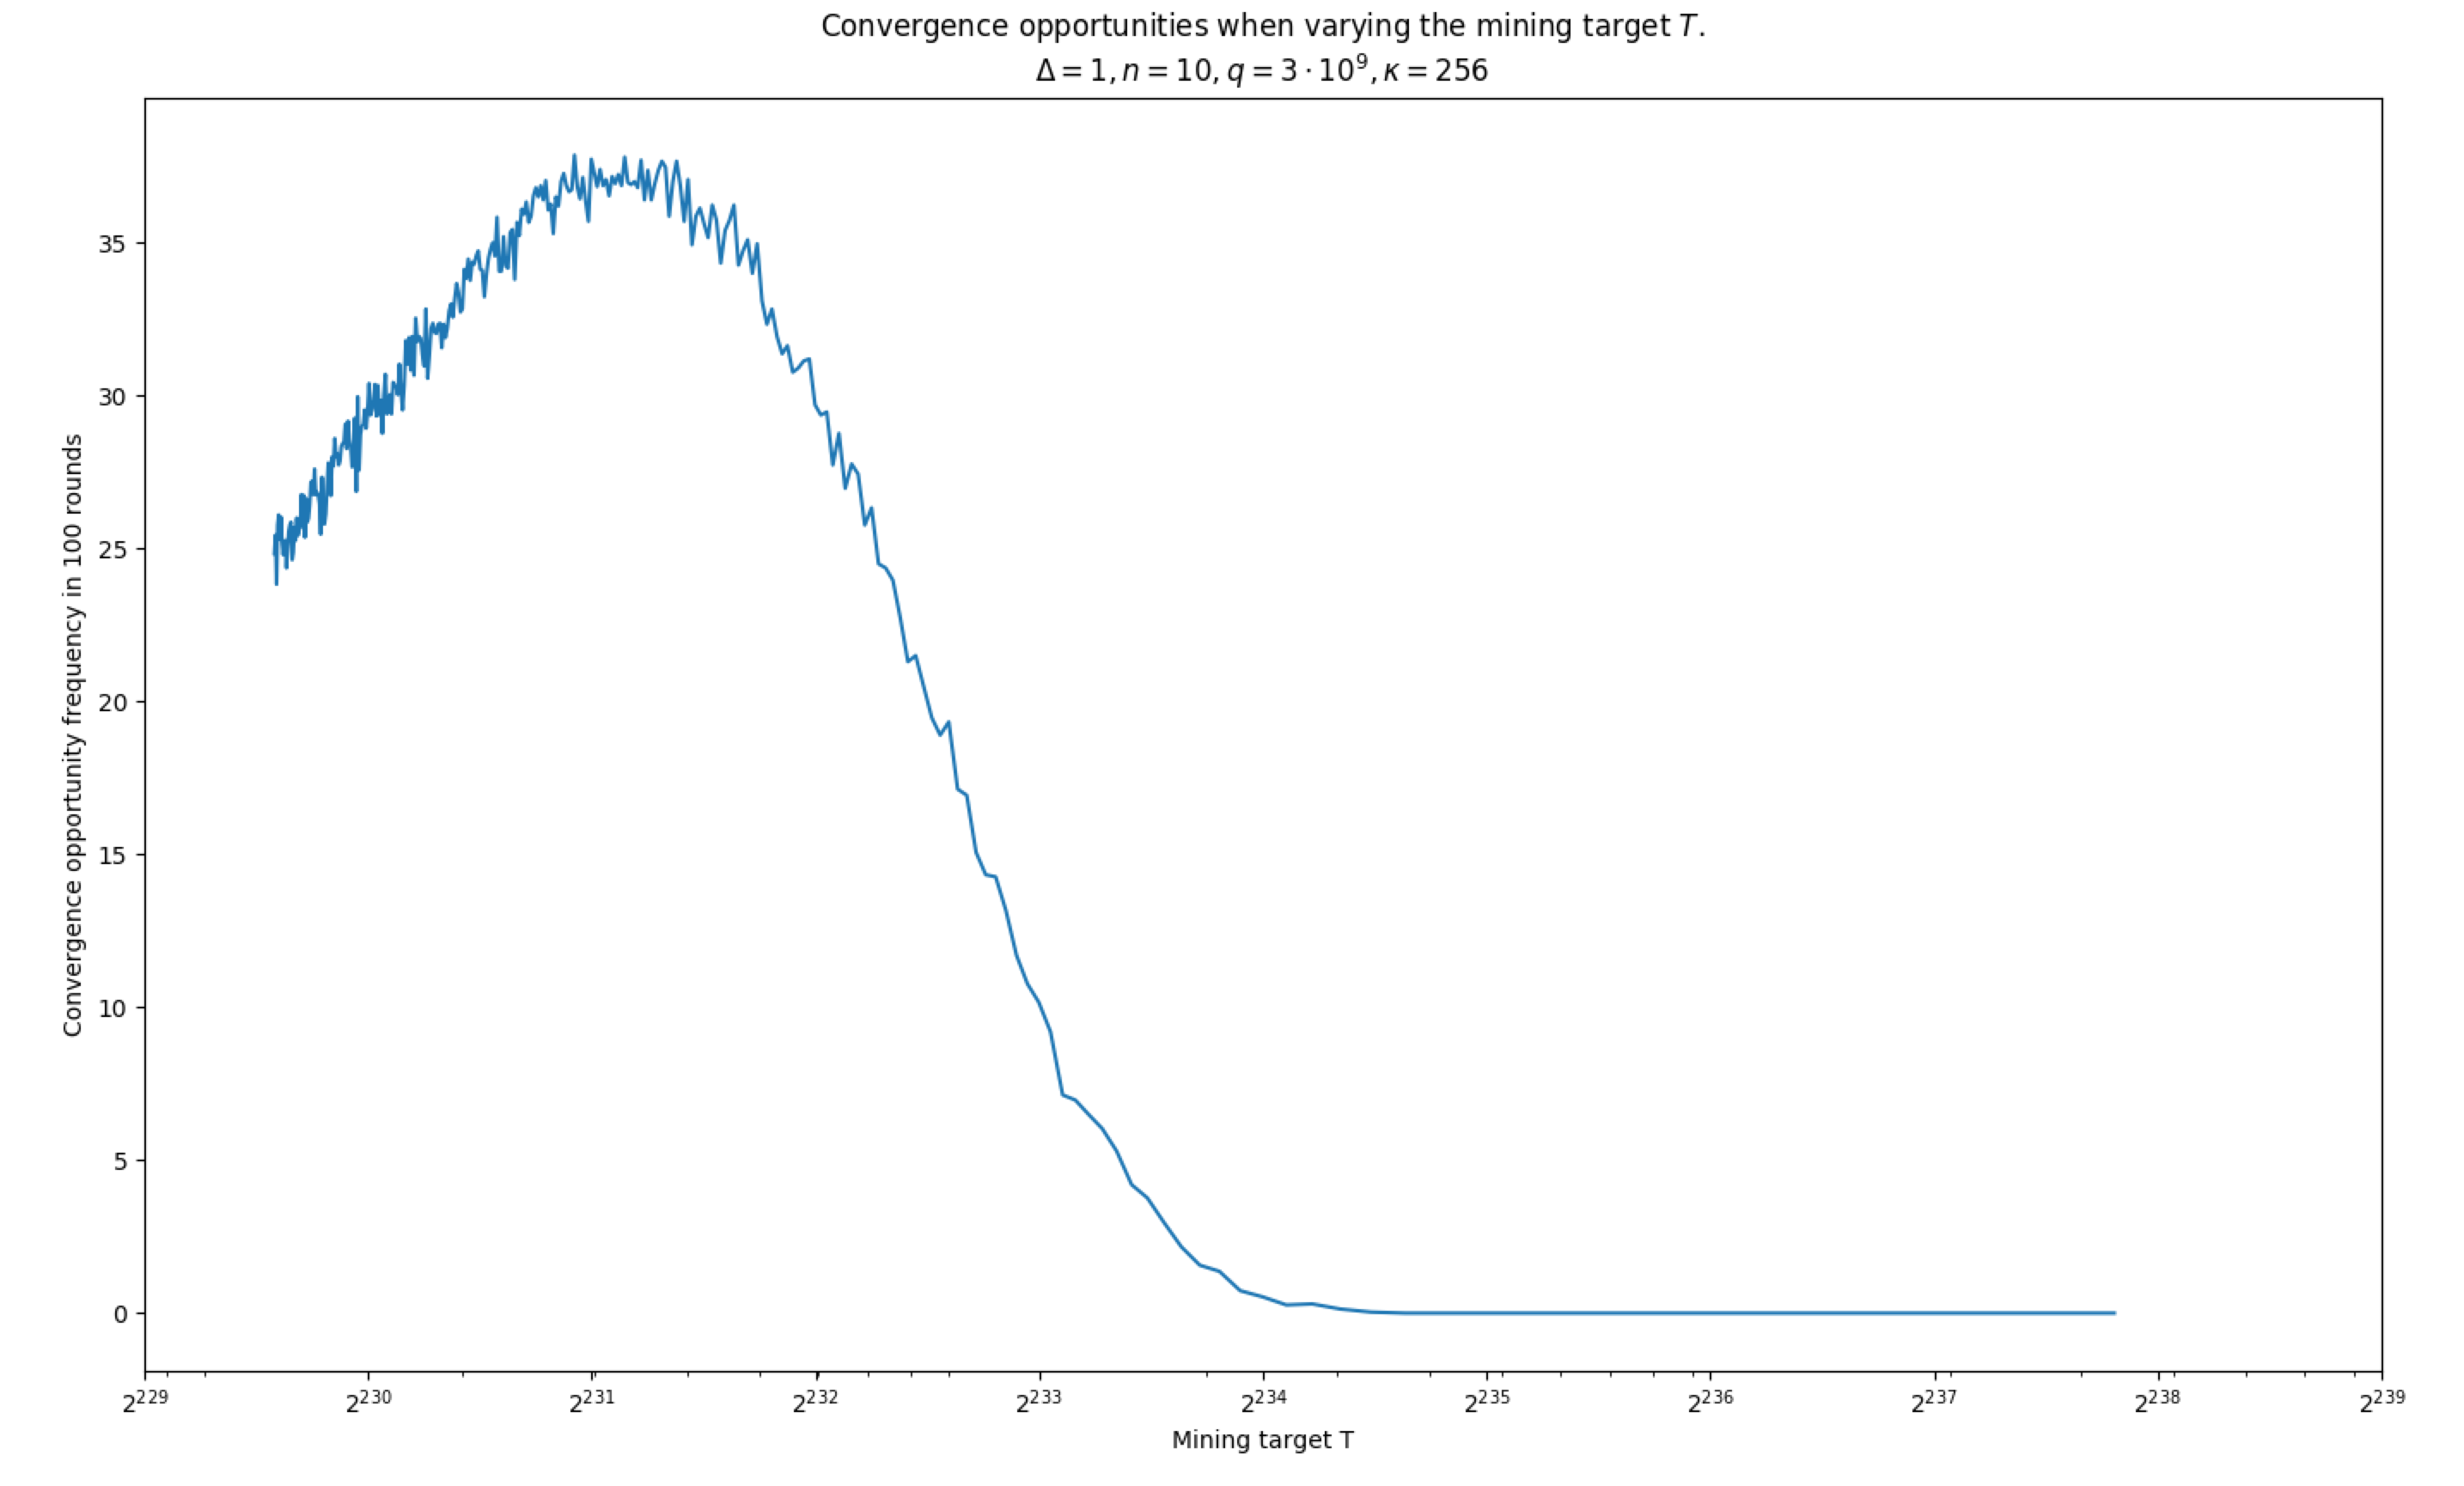
\includegraphics[scale=0.35]{figures/targetT.png}\]

\label{fig:convergence_opp_frequency}
\caption{Plot of convergence opportunity frequency versus target $T$}
\end{figure}

\section*{Problems}

\begin{problems}
  \item Implement Algorithm~\ref{alg.selfish-simulation} in your favourite programming language,
        and run it for values $t, n, c, m$ of your choice. Can you reproduce the results described
        in the text?
\end{problems}

\section*{Further Reading}

The Nakamoto Race was explored in Satoshi's Bitcoin paper. There, he analyzed the probability of
the success of a minority adversary mounting the Nakamoto Race attack against a majority of honest
parties. This is the only attack that Satoshi analyzed. He did not prove that his protocol is secure
against all adversaries. The longest chain protocol was analyzed and proven secure against \emph{all}
adversaries in the later work of the Bitcoin Backbone, which we explore in the later chapters of this
book.

In an even later work from 2020,
\emph{Everything is a Race and Nakamoto Always Wins~\cite{nakamoto-wins}},
the authors discuss hod Satoshi has been right all along, but we did not know it:
In fact, \emph{any} mining attack an adversary can possibly perform is roughly equivalent
to a Nakamoto Race.

While the Fan-Out was known to Nakamoto, but was made precise in the Bitcoin Backbone line of
work, where they argue that

\begin{quote}
$f$ cannot be too large, because [this would mean] that uniquely
successful rounds will not produce sufficiently many PoW's to overcome the PoW's
produced by the adversary.
\end{quote}
